\section{INTRODUÇÃO}

A dilatação térmica é um fenômeno físico que descreve a variação nas dimensões de um corpo (sólido, líquido ou gás) quando sua temperatura é alterada. A maioria dos materiais se expande quando aquecida e se contrai quando resfriada. Este fenômeno é de suma importância em diversas aplicações de engenharia, desde a construção de pontes e ferrovias até o design de componentes eletrônicos.

No caso dos sólidos, a dilatação pode ser linear, superficial ou volumétrica. A dilatação linear, foco deste experimento, refere-se à mudança no comprimento de um material. Teoricamente, a variação de comprimento $\Delta L$ de um material sólido com um comprimento inicial $L_0$ submetido a uma variação de temperatura $\Delta T$ é dada pela relação:
\begin{equation}
\Delta L = \alpha \cdot L_0 \cdot \Delta T
\label{eq:dilatacao_linear}
\end{equation}
\addtoequationlist{Dilatação Linear}
Onde $\alpha$ é o coeficiente de dilatação linear, uma propriedade intrínseca de cada material que quantifica sua tendência a dilatar ou contrair. Materiais diferentes possuem coeficientes de dilatação linear distintos. A unidade de $\alpha$ é tipicamente por grau Celsius ($^\circ C^{-1}$) ou por Kelvin ($K^{-1}$).

Este experimento, conforme ilustrado na Figura \ref{fig:esquema_montagem}, tem como objetivo determinar o coeficiente de dilatação linear ($\alpha$) de diferentes materiais (latão, alumínio e aço) através da medição da variação de comprimento de tubos metálicos quando aquecidos por vapor d'água. A comparação dos valores experimentais com os valores tabelados nos permitirá calcular o erro relativo, avaliando a precisão do nosso método.

\begin{figure}[H]
    \centering
    \caption{Esquema de montagem do Dilatômetro}
    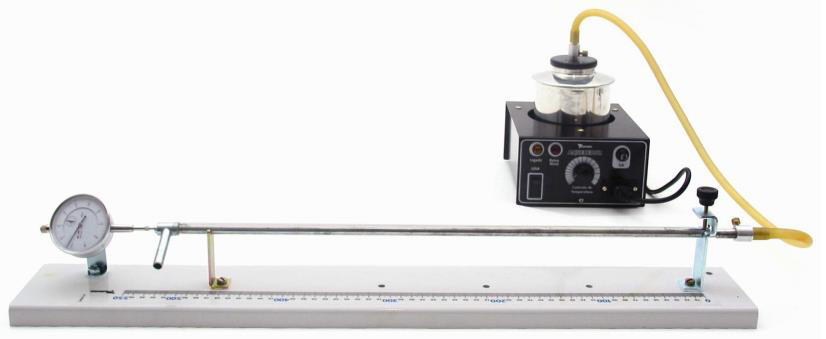
\includegraphics[width=0.7\linewidth]{figuras/esquema.png}
    \fonte{\citeonline{roteiro}}
    \label{fig:esquema_montagem}
\end{figure}

Os objetivos específicos deste experimento são:
\begin{enumerate}
    \item Realizar a montagem do dilatômetro e operar o gerador de vapor de forma segura e eficaz.
    \item Medir o comprimento inicial, as temperaturas inicial e final, e a dilatação dos corpos de prova de diferentes materiais.
    \item Calcular o coeficiente de dilatação linear ($\alpha$) para cada material com base nas medições.
    \item Comparar os valores experimentais de $\alpha$ com os valores tabelados e determinar o erro relativo.
    \item Discutir as fontes de incerteza e possíveis melhorias no procedimento experimental.
\end{enumerate}